\section{Ergebnisse}
\label{sec:ergebnisse}

Als Ergebnis der Versuchsdurchführung erhielt man lediglich das Spektrum welches in Abb. \ref{fig:spektrum_original} dargestellt ist. Die Beschriftung der einzelnen Peaks mit Buchstaben erfolgte im manuell im Rahmen der Auswertung dieses Spektrums.

\begin{figure}[h!]
		\centering
		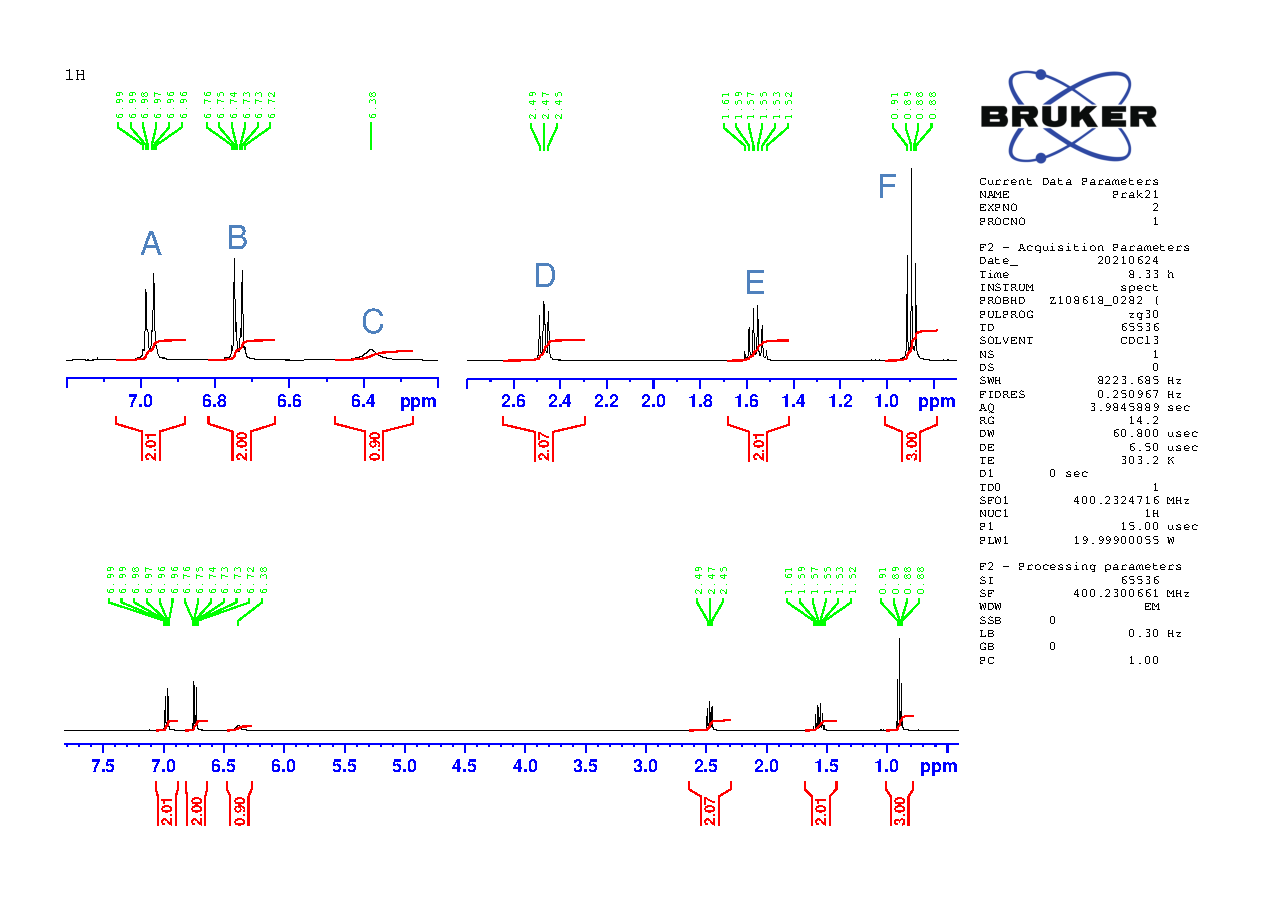
\includegraphics[page=1, width=\textwidth]{dokumente/spektrum_original.pdf}
		\caption{aufgenommenes ${}^1$H-NMR-Spektrum der unbekannten Probe}
		\label{fig:spektrum_original}
\end{figure}
\FloatBarrier
